\documentclass{beamer}
\usepackage[utf8]{inputenc}
\usepackage[T2A]{fontenc}
\usepackage[english, russian]{babel}
%\usepackage[sfdefault, light]{roboto}
\usepackage{epstopdf}
\usepackage[font={footnotesize}, labelfont={footnotesize}]{caption}
\usepackage[font={footnotesize}, labelfont={footnotesize}]{subcaption}
\usepackage{bm}
\usepackage[absolute,overlay]{textpos}
  \setlength{\TPHorizModule}{1mm}
  \setlength{\TPVertModule}{1mm}

\usepackage{tikz}

% Listings
\usepackage{listings}
\definecolor{codegreen}{rgb}{0,0.6,0}
\definecolor{codegray}{rgb}{0.5,0.5,0.5}
\definecolor{codepurple}{rgb}{0.58,0,0.82}
\definecolor{backcolour}{rgb}{0.95,0.95,0.92}
 
\lstdefinestyle{pythonstyle}{
    backgroundcolor=\color{backcolour},   
    commentstyle=\color{codegreen},
    keywordstyle=\color{magenta},
    numberstyle=\tiny\color{codegray},
    stringstyle=\color{codepurple},
    basicstyle=\scriptsize,
    breakatwhitespace=false,         
    breaklines=true,                 
    captionpos=b,                    
    keepspaces=true,                 
    numbers=left,                    
    numbersep=5pt,                  
    showspaces=false,                
    showstringspaces=false,
    showtabs=false,                  
    tabsize=2
}
\lstset{style=pythonstyle, language=Python}

\graphicspath{ {images/} }
\setbeamertemplate{caption}{\raggedright\insertcaption\par}
\def\figurename{}

\title{Базовые модели машинного обучения:\\кластеризация}
\date[\today]{Практика по дисциплине <<Технологии ИИ>>\\\today}
\author[Anton]{Гирдюк Дмитрий Викторович\\Першин Антон Юрьевич, Ph.D.\\Никольская Анастасия Николаевна}

\institute{Программа <<Большие данные и распределенная цифровая платформа>>\\Санкт-Петербургский государственный университет}

\usetheme{tonythequick}

%%%%%%%%%%%%%%%%%%%%%%%%%%%%%%%%%%%%%%%%

\usepackage[ruled,vlined]{algorithm2e}
\usepackage{wrapfig}
\usepackage{pgfplots}


% \usepackage[style=gost-numeric,
%   backend=biber,
%   language=auto,
%   hyperref=auto,
%   autolang=other,
%   sorting=none
% ]{biblatex}

% \renewcommand*{\newblockpunct}{
%     \addperiod\space\bibsentence}

% \addbibresource{bibliography.bib}

% \setbeamertemplate{bibliography item}{\insertbiblabel}

% \usepackage{etoolbox}
% \patchcmd{\thebibliography}{\section*{\refname}}{}{}{}


\begin{document}

\begin{frame}
\titlepage
\end{frame}

\setcounter{framenumber}{0}

\section{}

\begin{frame}{Обучение без учителя}
    \small

    \begin{itemize}
        \item \textit{Обучение без учителя} (unsupervised learning)~-- это тип машинного обучения, который ищет ранее необнаруженные закономерности в наборе данных без ранее существовавших меток и с минимальным или полностью отсутствующим контролем человека.
    
        \item Задача обучения без учителя покрывает не только \textit{кластеризацию}, но и
        \textit{
        \begin{itemize}
            \item поиск ассоциативных правил
            \item заполнение пропущенных значений
            \item поиск аномалий
            \item сокращение размерности и визуализация данных
        \end{itemize}
        }
    \end{itemize}
\end{frame}

\begin{frame}{Постановка задачи кластеризации}
    \small

    \begin{itemize}
        \item \textit{Кластерный анализ} или \textit{кластеризация}~-- это задача группировки набора объектов таким образом, чтобы объекты в одной группе (называемой кластером) были более похожи (в некотором смысле) друг на друга, чем на объекты в других группах (кластерах).

        \item Проще говоря, имеем
        \begin{itemize}
            \item Пространство объектов $X = \{ x_i\}_{i=1}^n, x_i \in \mathbb{R}^m$ и выборку из него $\widehat X$
            \item Мера расстояния между объектами $\rho: X \times X \rightarrow R^+$
            \end{itemize}
            Хотим получить
            \begin{itemize}
                \item Множество групп/кластеров $Y = \{ y_i \}_{i=1}^n, y_i \in \mathbb{N}$
                \item Алгоритм кластеризации $\alpha: X \rightarrow Y$
            \end{itemize}
        \end{itemize}
\end{frame}

\begin{frame}{Приложения}
    \small
    
    \begin{itemize}
        \item Разделение на группы с целью упрощения работы (отдельные модели для каждой группы).
        \item Сокращение объемов наблюдений и сжатие данных (например, квантизация нейронных сетей).
        \item Выделение новизны/аномалий.
        \item Построение иерархии/таксономии объектов.
    \end{itemize}
\end{frame}

\begin{frame}{Примеры кластеризации}
    \small

    \begin{figure}
        \centering
        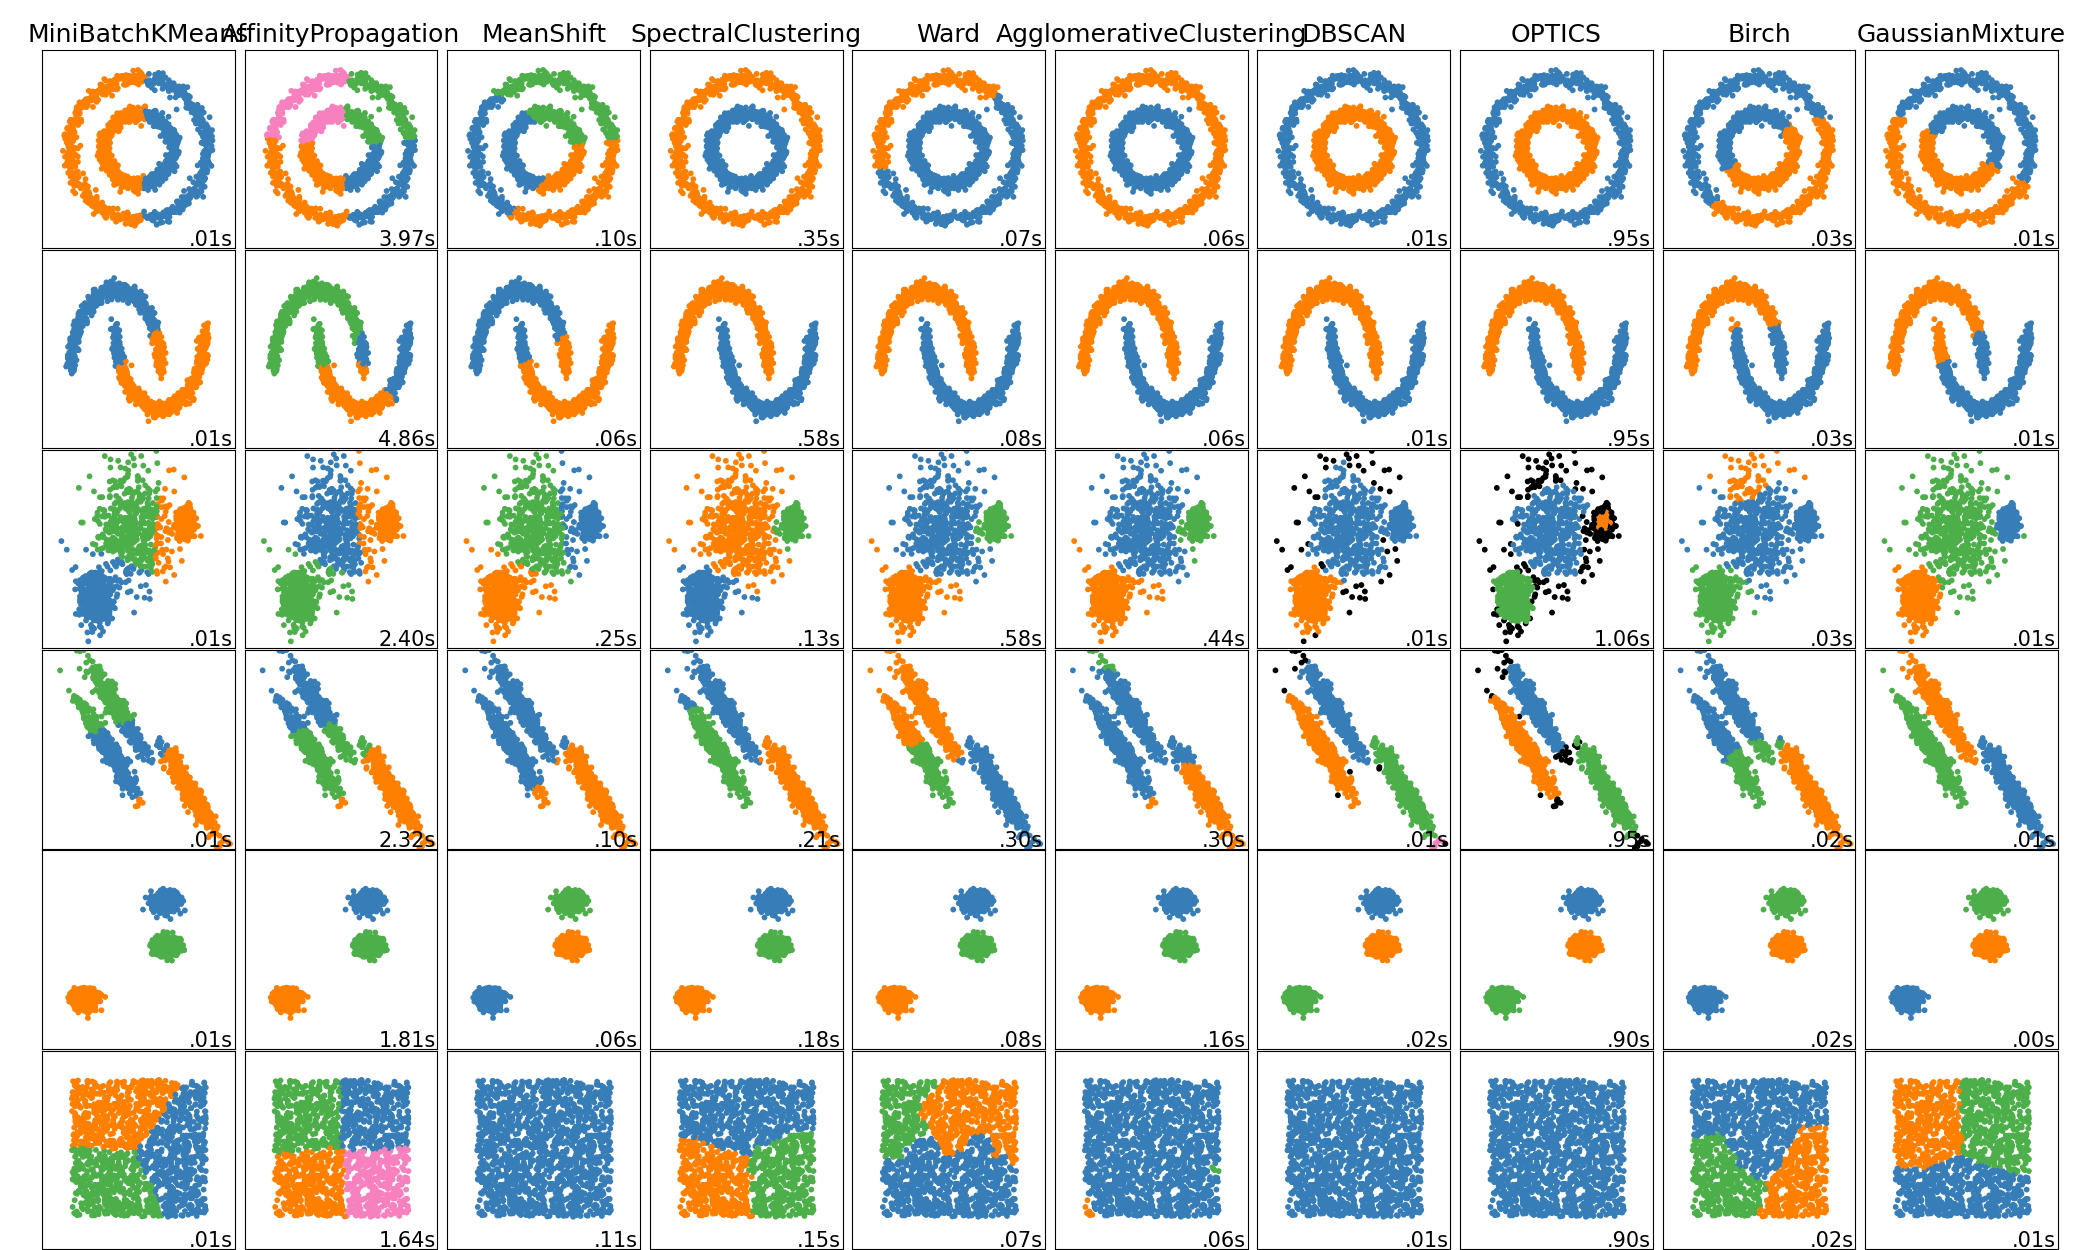
\includegraphics[width=\linewidth]{sklearn_clust.png}
        
        \href{https://scikit-learn.org/stable/modules/clustering.html}{Источник изображения}
    \end{figure}
\end{frame}

\begin{frame}{Классификация алгоритмов}
% ~\cite{FAHAD2014,Tiruveedhula2016,  BENABDELLAH2019}
    \small
    
    В большинстве источников выделяют пять групп алгоритмов
    \begin{itemize}
        \item \textit{Основанные на центроидах} (centroid based): \textbf{k-means}, k-modes, k-medoids, \textbf{Meanshift}, FCM, Affiniy propagation.
        \item \textit{Иерархические} (hierarchical): \textbf{агломеративные} (Ward, single/average/complete linkage), BIRCH, на основе теории графов (выделение связных компонент и минимальное остовное дерево), \textbf{Spectral Clustering}, CURE, ROCK, Chameleon, Echidna, SNN, CACTUS, GRIDCLUST.
        \item \textit{Основанные на плотности} (density based): \textbf{DBSCAN}, OPTICS, DBCLASD, GDBSCAN, DENCLU, SUBCLU.
        \item \textit{Сеточные} (grid based): STING, Wave cluster, BANG, CLIQUE, OptiGrid, MAFIA, ENCLUS, PROCLUS, ORCLUS, FC, STIRR.
        \item \textit{Основанные на модели данных} (model based): \textbf{Expectation Maximization} (EM), COBWEB, CLASSIT, SOM.
    \end{itemize}

\end{frame}

\begin{frame}{k-means}
    \small
    
    \begin{itemize}
        \item Алгоритм k-means -- один из самых простых и популярных алгоритмов кластеризации, заключающийся в поиске заранее заданного числа кластеров путем минимизации суммы квадратов внутрикластерных расстояний между точками кластеров и соответствующих им центроидами.
        \item Получаемая оптимизационная задача вычислительно трудна (NP-сложная), однако разработано достаточно много эвристических алгоритмов, позволяющих достаточно быстро отыскать локальный минимум.
    \end{itemize}
\end{frame}

\begin{frame}{Формальное определение}
    \small
    
    \begin{itemize}
        \item Пусть $S=\{ S_1, S_2, \ldots, S_k\}$ есть разбиение выборки на $k$ непересекающихся множеств.
        \item Тогда задача минимизации суммы квадратов внутрикластерных расстояний может быть записана следующим образом
        $$\arg \min_{S} \sum_{i=1}^k \sum_{x \in S_i} ||x - \mu_i||^2 = \arg \min_{S} \sum_{i=1}^k \left | S_i \right | \text{Var} S_i,$$
        $$\mu_i = \frac{1}{\left | S_i \right |} \sum_{x \in S_i} x$$
    \end{itemize}
\end{frame}

\begin{frame}{k-means: описание алгоритма Ллойда}
    \small
    
    \begin{enumerate}
        \item Зафиксировав число кластеров, произвольным образом инициализируем $k$ центроид. Это могут быть наблюдения из выборки, произвольные точки в пространстве данных или что-нибудь более умное, вроде использования эмпирической плотности распределения данных (k-means++).
        \item Относим каждое наблюдение к кластеру, чей центроид (центр тяжести) находится к наблюдению ближе всего.
        \item Обновляем центроиды с учетом всех входящих в каждый кластер наблюдений.
        \item Повторяем шаги 2 и 3 фиксированное количество раз или до тех пор, пока все центроиды не стабилизируются (т.е. изменяются по норме не больше заранее заданного $\varepsilon$).
    \end{enumerate}
        
\end{frame}

\begin{frame}{k-means: пример}
    \small
    
    \begin{figure}
        \centering
        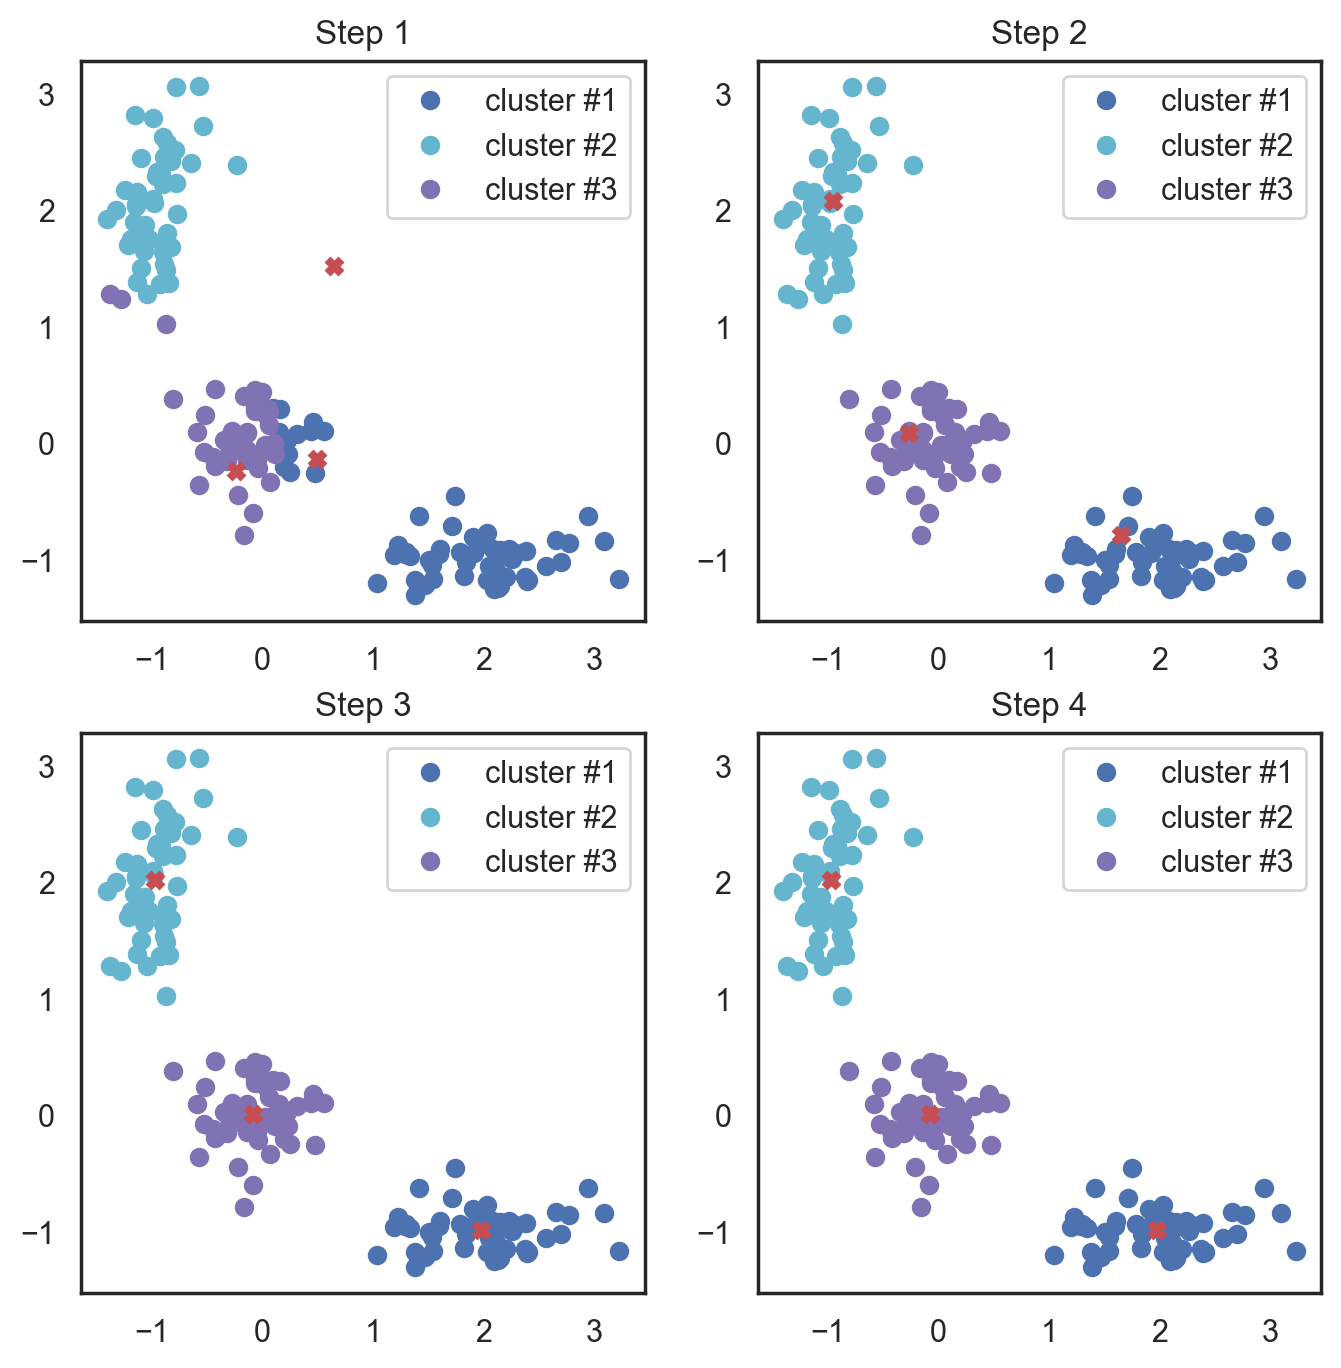
\includegraphics[width=0.6\linewidth]{kmeans.png}
        
        \href{https://mlcourse.ai/book/topic07/topic7_pca_clustering.html
}{Источник изображения}
    \end{figure}
\end{frame}


%%%%%%
\begin{frame}{k-means: алгоритм Ллойда}
    \small
    
    \begin{algorithm}[H]
        \SetKwData{Left}{left}\SetKwData{This}{this}\SetKwData{Up}{up}
        \SetKwFunction{Union}{Union}\SetKwFunction{FindCompress}{FindCompress}
        \SetKwInOut{Input}{input}\SetKwInOut{Output}{output}
        
        \Input{Выборка $X = \left \{ x_1, \ldots, x_n \right \}$, количество кластеров $k$ и $\varepsilon$}
        Произвольным образом инициализируем $k$ центроид $\mu_i$\\
        \While{True}{
            Относим наблюдения к ближайшим центроидам:
            $$S_i := \left \{ x_p : ||x_p - \mu_i||^2 \leqslant || x_p - \mu_j ||^2, 1 \leqslant j \leqslant k  \right \}$$\\
            Обновляем центроиды:
            $$\mu_i = \frac{1}{\left | S_i \right |} \sum_{x \in S_i} x$$\\
            \If{$\max_{i, j} | g_{ij} - g^0_{ij}| < \varepsilon$}{Завершить работу}
        }
        \caption{k-means}
    \end{algorithm}
\end{frame}


\begin{frame}{k-means: обсуждение}
    \small
    
    \begin{itemize}
        \item Отличное базовое решение.
        \item Алгоритм метрический, потому либо нормализуем данные, либо определяем специальную метрику.
        \item Алгоритм прост и понятен, имеет большое количество всевозможных обобщений (k-medians, k-medoids, k-means++ и т.д.).
        \item Не гарантируется достижение глобального минимума суммарного квадратичного отклонения, а только одного из локальных минимумов. Кроме того, полученные кластеры зачастую стремятся иметь сферическую форму ввиду вида целевой функции.
        \item Результат зависит от выбора исходных центров кластеров, их оптимальный выбор неизвестен. Чаще всего алгоритм запускают несколько раз и выбирают то разбиение, которое показало наименьшее значение целевой функции.
    \end{itemize}
\end{frame}

\begin{frame}{k-means: эвристика выбора числа кластеров}
    \small
    
    \begin{itemize}
        \item Число кластеров необходимо задавать заранее. На практике производят разбиения для различных значений $k$, строят график значений целевой функции и ищут такое значение $k$, после которого значение целевой функции перестает сильно изменяться (так называемый <<метод локтя>>).
    \end{itemize}
    
    \begin{figure}
        \centering
        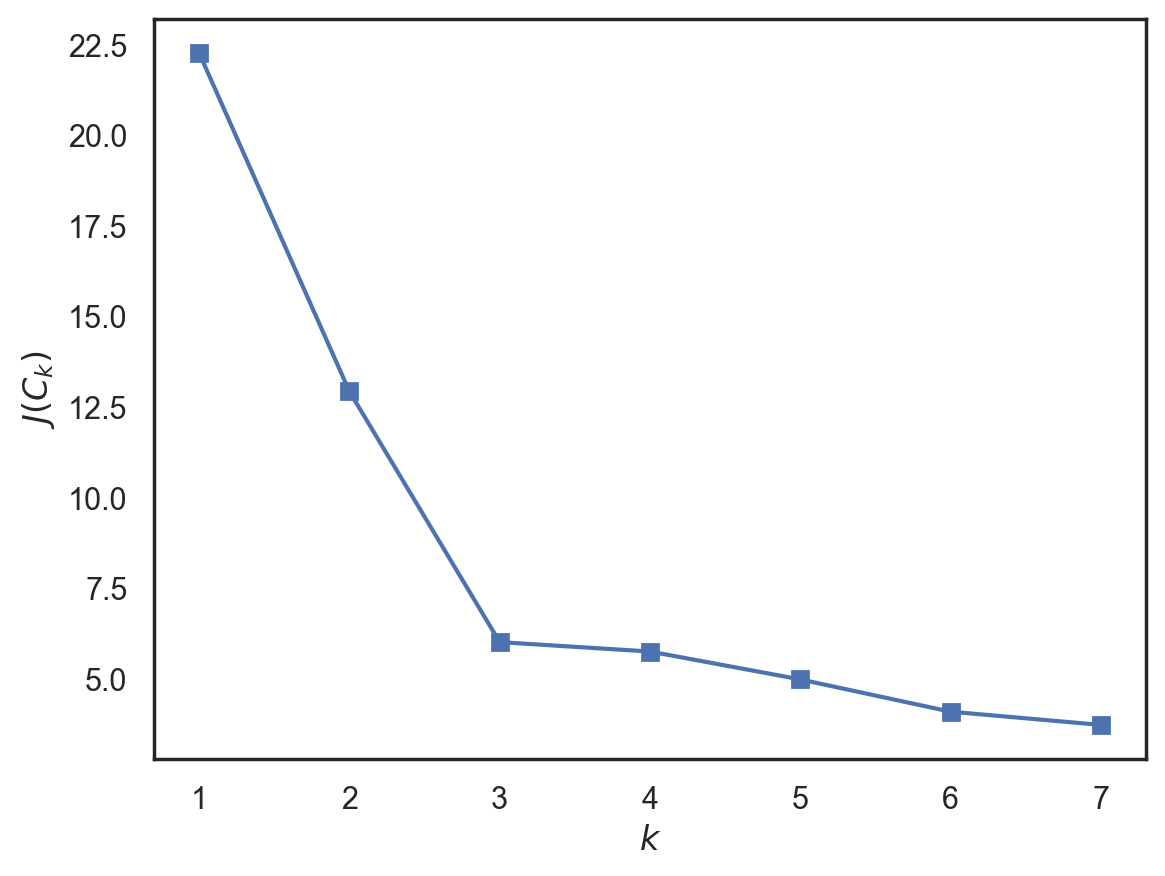
\includegraphics[width=0.6\linewidth]{elbow_method.png}
        
        \href{https://mlcourse.ai/book/topic07/topic7_pca_clustering.html
}{Источник изображения}
    \end{figure}
\end{frame}

\begin{frame}{k-means: sklearn}
    \small

    \begin{itemize}
        \item k-means реализован в sklearn'е.
        \item Кроме числа кластеров n\_clusters основными гиперпараметрами являются:
        \begin{itemize}
            \item init. Метод инициализации центроид. k-means++ (стандартный), рандомный и определенный пользователем.
            \item n\_init. Количество запусков алгоритма (было описано ранее на слайдах).
            \item algorithm. Алгоритм Ллойда или Элкана. Второй является модификацией алгоритма Ллойда: ускорение работы путем исключения некоторого числа вычислений расстояний за счет использования неравенства треугольника.
        \end{itemize}       
    \end{itemize}
\end{frame}

\begin{frame}{DBSCAN}
    \small
    
    \begin{itemize}
        \item Density-Based Spatial Clustering of Appliations with Noise (DBSCAN)~-- алгоритм кластеризации, основанный на плотности точек, изначально разработанный с целью кластеризации в базах данных, содержащих геометрические представления наблюдений.
        \item Основными преимуществами алгоритма авторы выделили минимальную необходимость понимания предметной области данных при подборе гиперпараметров метода, а также способность обнаруживать кластеры произвольной формы.
        \item Алгоритм достаточно прост, наряду с k-means один из самых популярных.
    \end{itemize}
\end{frame}

\begin{frame}{DBSCAN: описание алгоритма}
    \small
    
     \begin{itemize}
        \item Алгоритм имеет 2 гиперпараметра: величина окрестности точки $\varepsilon$ и минимальное количество наблюдений в окрестности $MinPts$
        \item При кластеризации точка может быть причислена к одному из 3 типов: 
            \begin{itemize}
                \item корневая: в ее $\varepsilon$-окрестности не менее $MinPts$ точек
                \item граничная: в ее $\varepsilon$-окрестности меньше $MinPts$ точек, но среди них есть как минимум одна корневая
                \item шумовая: не корневая и не граничная
            \end{itemize}
        \end{itemize}
\end{frame}

\begin{frame}{DBSCAN: иллюстрация типов наблюдений}
    \small
       
    \begin{figure}
        \centering
        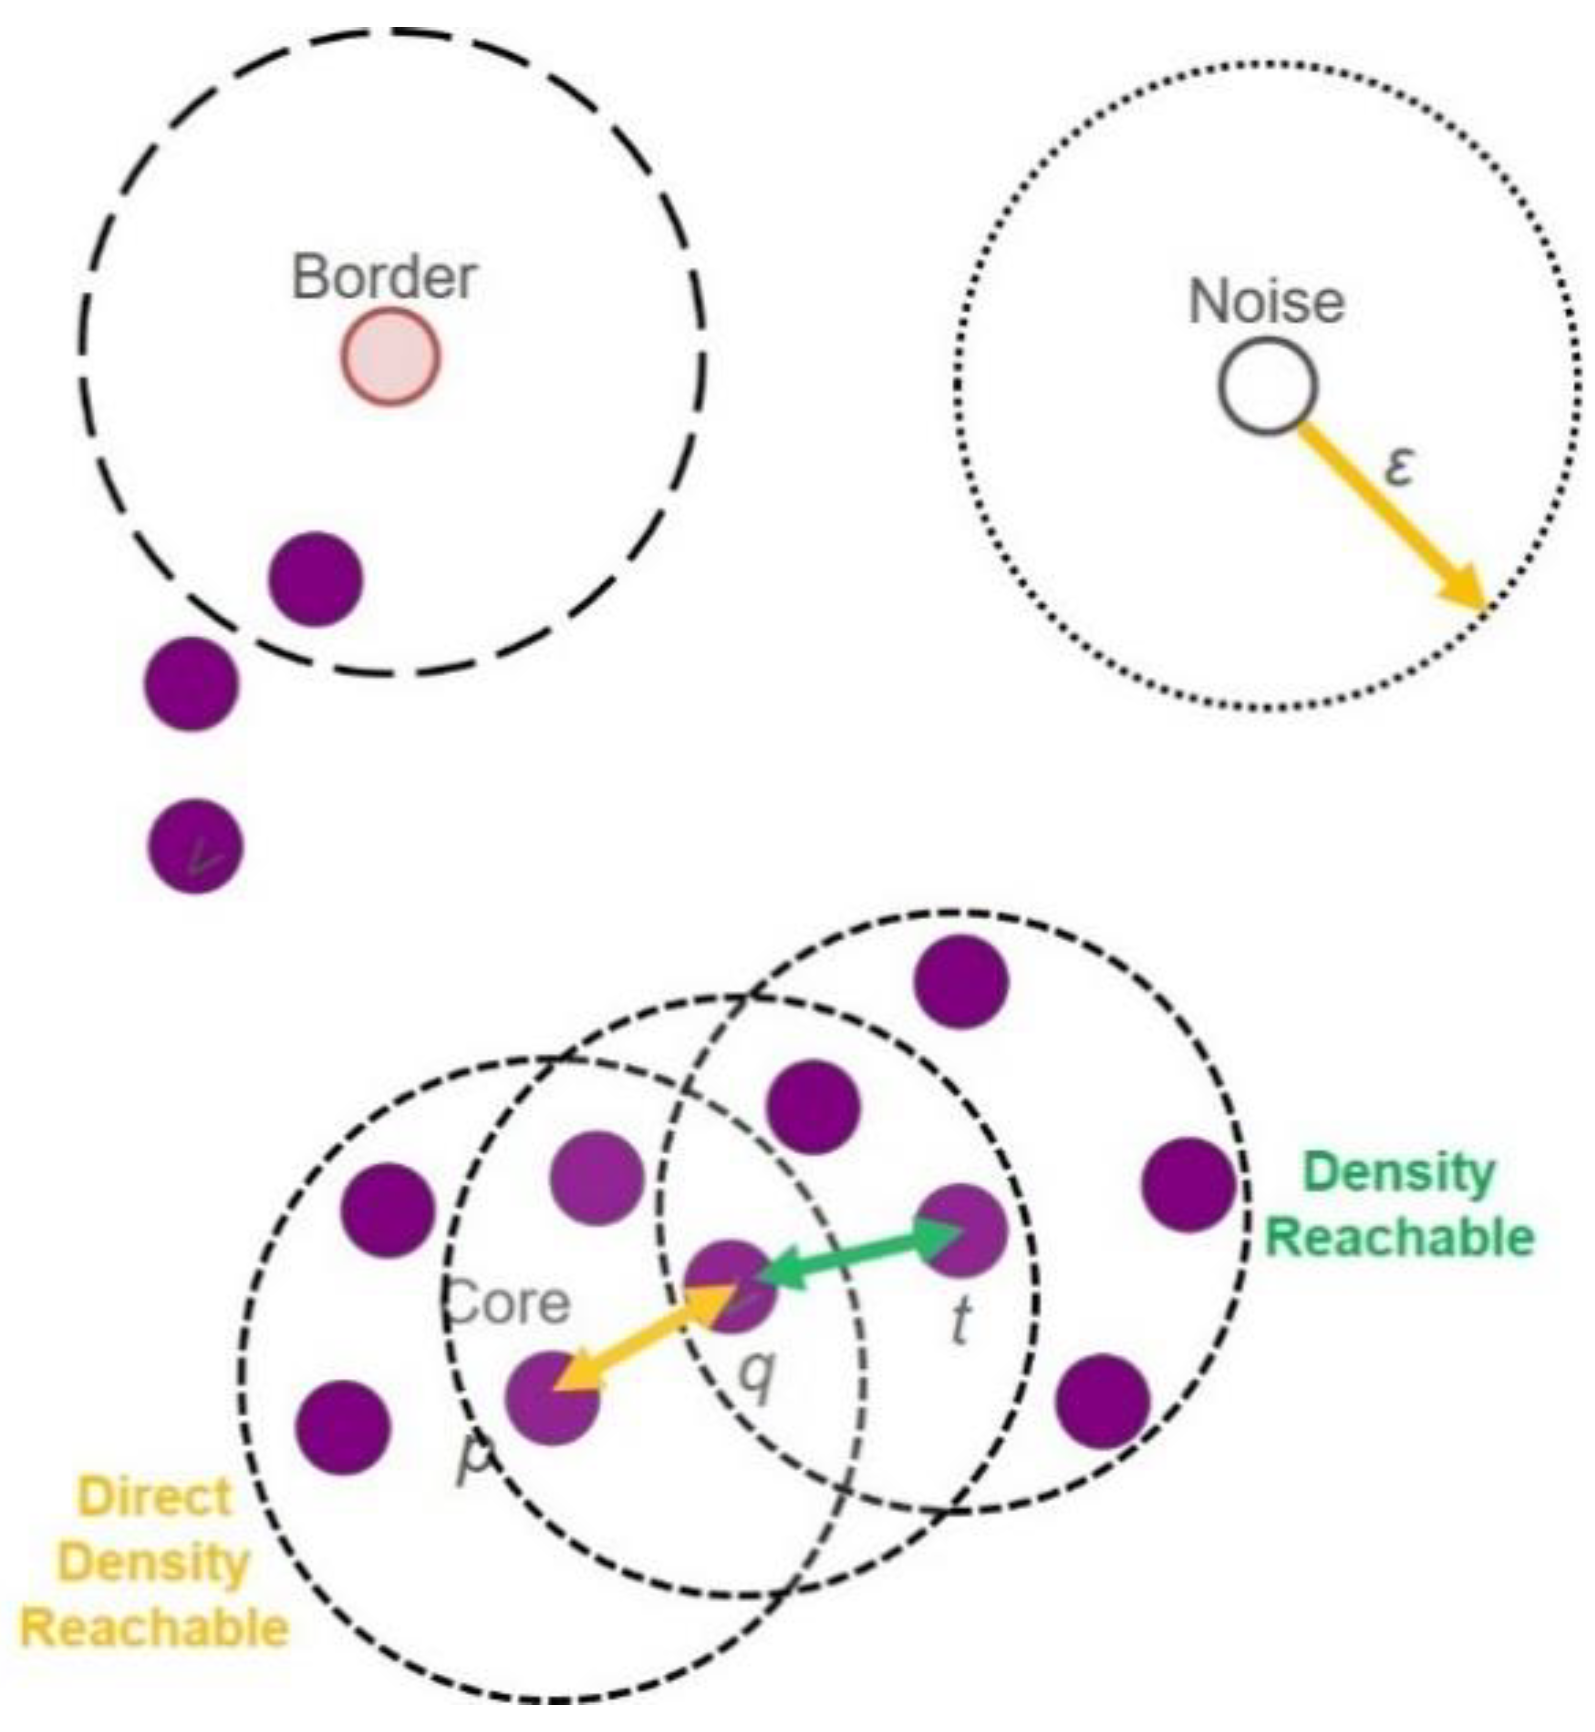
\includegraphics[width=0.6\textwidth]{dbscan.png}
        
        \href{https://www.mdpi.com/2076-3417/9/20/4398}{Источник изображения}
    \end{figure}
\end{frame}

\begin{frame}{DBSCAN: алгоритм}
    \small
    
    \begin{algorithm}[H]
        \SetKwData{Left}{left}\SetKwData{This}{this}\SetKwData{Up}{up}
        \SetKwFunction{Union}{Union}\SetKwFunction{FindCompress}{FindCompress}
        \SetKwInOut{Input}{input}\SetKwInOut{Output}{output}
        
        \Input{Выборка $X = \left \{ x_1, \ldots, x_n \right \}$, параметры $\varepsilon$ и $MinPts$}
        $U = X, K = \emptyset, a = 0, a_1, \dots, a_n = -1$\;
        \While{$U \neq \emptyset$}{
        	Взять $x \in U$\;
        	\eIf{$|U_\varepsilon(x)|<MinPts$}{
        		Пометить $x$ как потенциально шумовую точку\;
        		}{
        			$K = U_\varepsilon(x), a=a+1$\;
                        \For{$x' \in K$}{
            			\eIf{$|U_\varepsilon(x)| \geq MinPts$}{
            				$K = K \cup U_\varepsilon(x')$\;
            			}{
            				пометить $x'$ как граничную точку кластера $K$\;
            			}
                        }
                        \lForEach{$x_i \in K$}{$a_i = a$}
        		      $U = U \setminus K$\;
        		}
        }
        \caption{DBASCAN}
    \end{algorithm}	
\end{frame}

\begin{frame}{DBSCAN: Подбор гиперпараметров}
    \small
    
    \begin{itemize}
        \item Общая идея состоит в построении графика, по ординате у которого расстояние до $MinPts$-го соседа, а по абсциссе -- точки, отсортированные в порядке увеличения этого расстояния.
        \item Существенный скачок в значении идентифицирует выбросы, посему задавая некоторый процент на их число можно определить $\varepsilon$. 
        \item Обычно строят несколько таких графиков для различных значений $MinPts$. 
        \item В некоторых источниках значение $MinPts$ предлагают выбирать равным $\text{dim}X + 1$, Где-то встречается $2 * \text{dim}X$
    \end{itemize}
\end{frame}

\begin{frame}{DBSCAN: sklearn}
    \small

    \begin{itemize}
        \item Есть реализация в sklearn'е. Кроме того, там же представлена модификация алгоритма под названием OPTICS, фактически отличающаяся от него тем, что задает интервал для значений $\varepsilon$, что позволяет выделять кластеры с различными плотностями.
        \item Основные гиперпараметры:
        \begin{itemize}
            \item eps и min\_samples. $\varepsilon$ и $MinPts$ соответственно.
            \item algorithm. Способ поиска соседей: брутфорс, ball-дерево, KD-дерево, и автоматический подбор подходящего с учетом обучающей выборки (дефолтное).
            \item leaf\_size. Максимальный размер листа в дереве, если выбрано ball/KD-дерево.
            \item metric и $p$. Метрику можно как реализовать самостоятельно, так и использовать из имеющегося: Минковского ($p$ -- ее параметр) и ее частные случаи (Чебышева и Манхэттенская).
        \end{itemize}       
    \end{itemize}
\end{frame}


% \begin{frame}[allowframebreaks]{Использованные источники}
%     \printbibliography[heading=none]
% \end{frame}


\end{document}
